
\section{GW}
\subsection{GW+2SOSEX-psd}
\begin{frame}
    \frametitle{Theory}
\begin{equation}
    \Sigma_{pp}^{G W+2 \mathrm{SOSEX}-\mathrm{psd}}(\omega)=\sum_{k s} \frac{\left(w_{s, \rm LDA}^{p k}+\tilde{w}_{s, \rm LDA}^{p k}\right)^2}{\omega-\epsilon_k^{\rm LDA}+\Omega_s^{\rm LDA}-\mathrm{i} \eta_{\Sigma}}+\sum_{c s} \frac{\left(w_{s, \rm LDA}^{p c}+\tilde{w}_{s, \rm LDA}^{p c}\right)^2}{\omega-\epsilon_c^{\rm LDA}-\Omega_s^{\rm LDA}+\mathrm{i} \eta_{\Sigma}}
\end{equation} \pause
with
\begin{equation}
    \tilde{w}_{s, \rm LDA}^{p c}=\sum_{a j} w_{s, \rm LDA}^{a j} \cdot\left[\frac{(p a|j c)}{\epsilon_a^{\rm LDA}-\epsilon_j^{\rm LDA}-\Omega_s^{\rm LDA}}+\frac{(p j | a c)}{\epsilon_a^{\rm LDA}-\epsilon_j^{\rm LDA}+\Omega_s^{\rm LDA}}\right] \pause
\end{equation}
Authors said they "found that the satellite structures in the spectral functions were very sensitive to the technical details, basis set, mean-field starting point"
\end{frame}
\begin{frame}
    \frametitle{14e19o}
    \begin{figure}
        \centering
        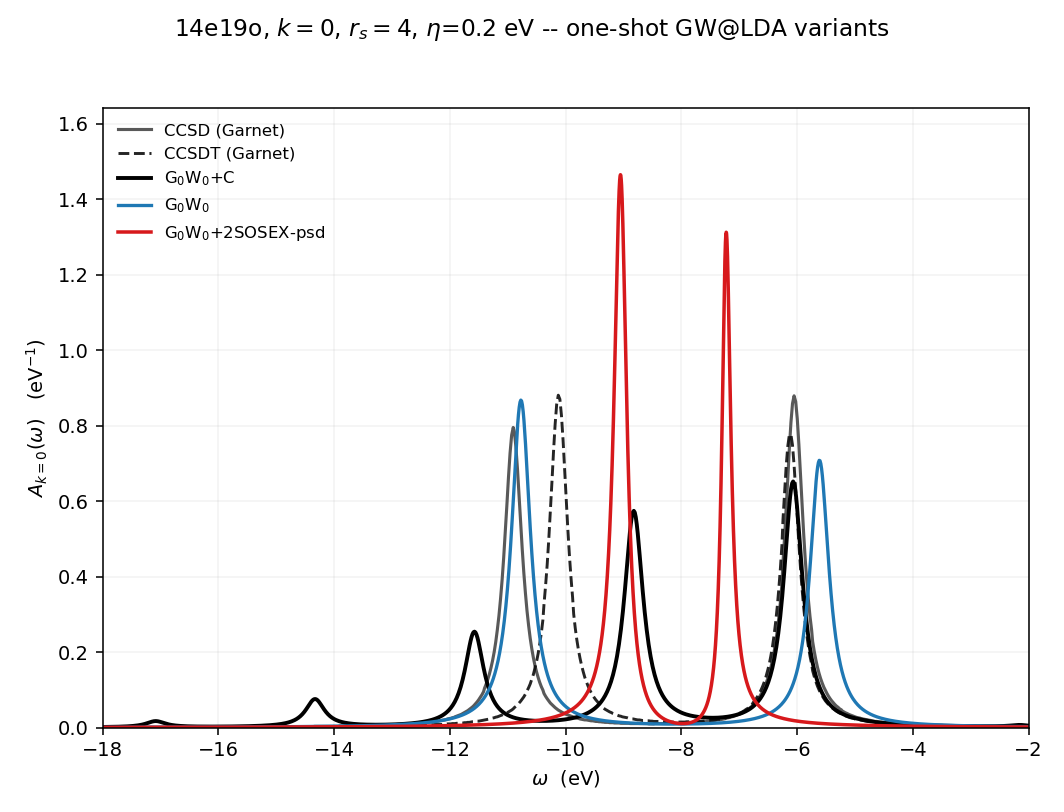
\includegraphics[width=0.9\textwidth]{26/9/9-09/k0_14e19o_drpa_lda_gwvar_lda.png}
\end{figure}
\end{frame}
\begin{frame}
    \frametitle{114e485o}
    \begin{figure}
        \centering
        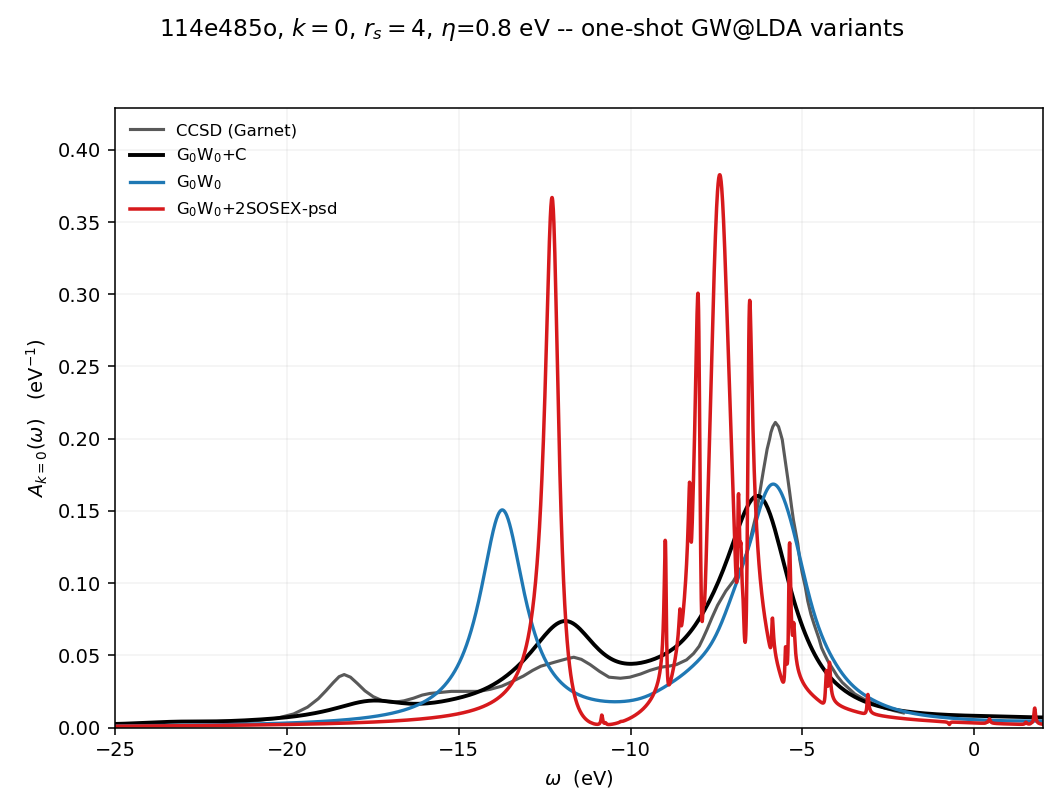
\includegraphics[width=0.9\textwidth]{26/9/9-09/k0_114e485o_drpa_lda_gwvar_lda.png}
\end{figure}
\end{frame}

\begin{frame}
    \frametitle{What we have for 114e485o}
    \begin{figure}
        \centering
        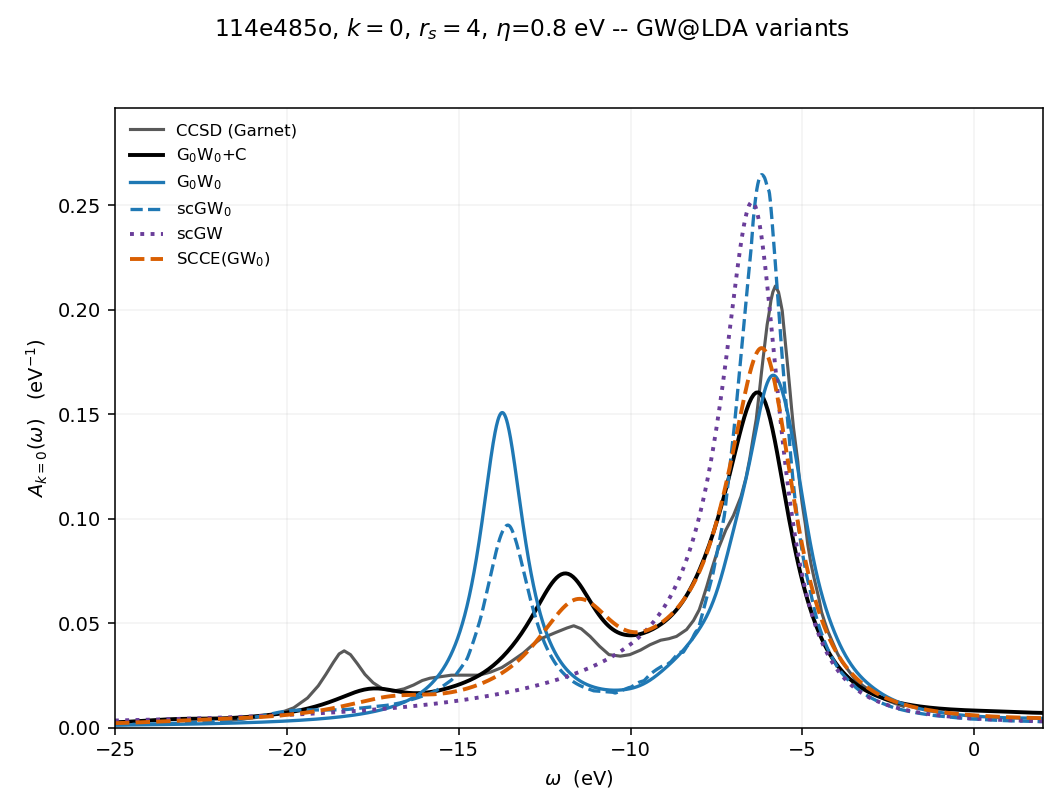
\includegraphics[width=0.9\textwidth]{26/9/9-09/k0_114e485o_drpa_lda_gwvar.png}
\end{figure}
\end{frame}
\begin{frame}
    \frametitle{G0W0+C}
    \begin{figure}
        \centering
        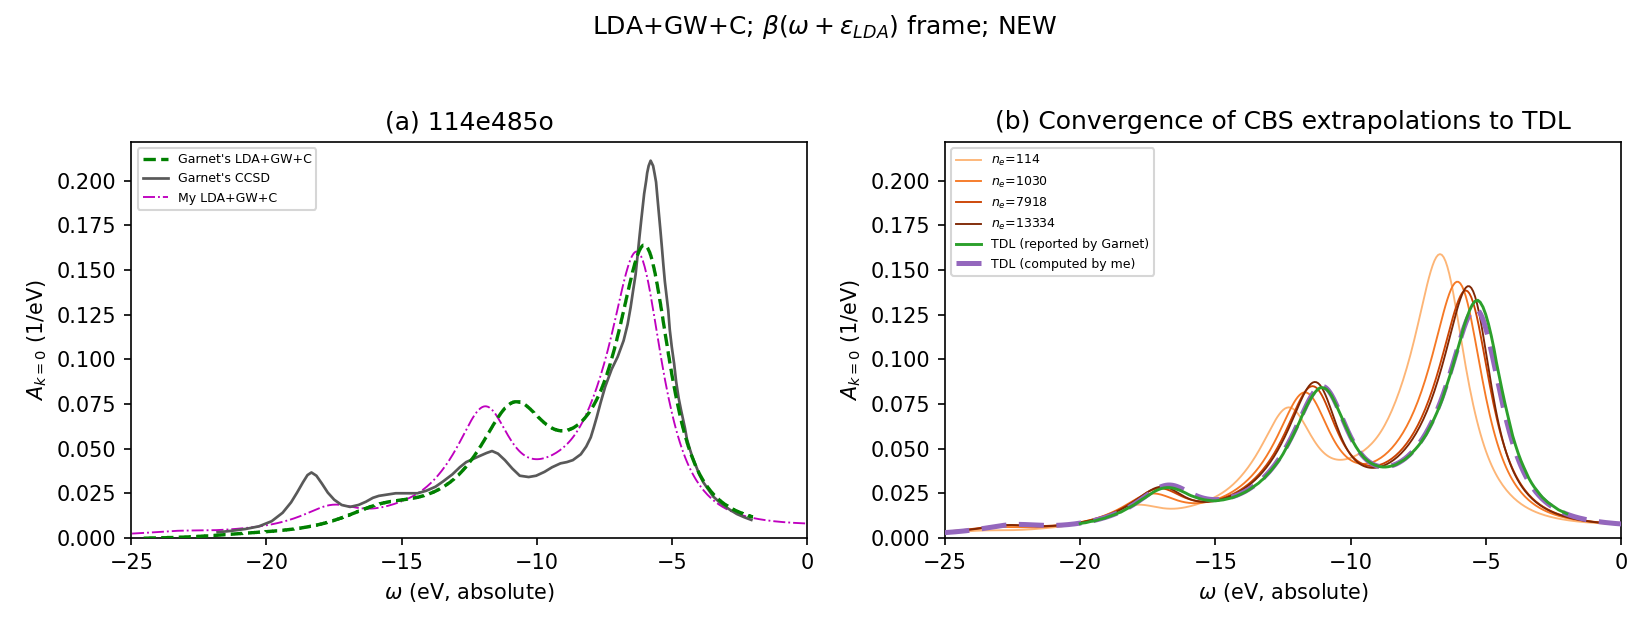
\includegraphics[width=\textwidth]{26/8/8-28/mcclain_gwc_compare_es0p0272.png}
\end{figure}
\end{frame}
\begin{frame}
    \frametitle{SCCE(GW0)}
    \begin{figure}
        \centering
        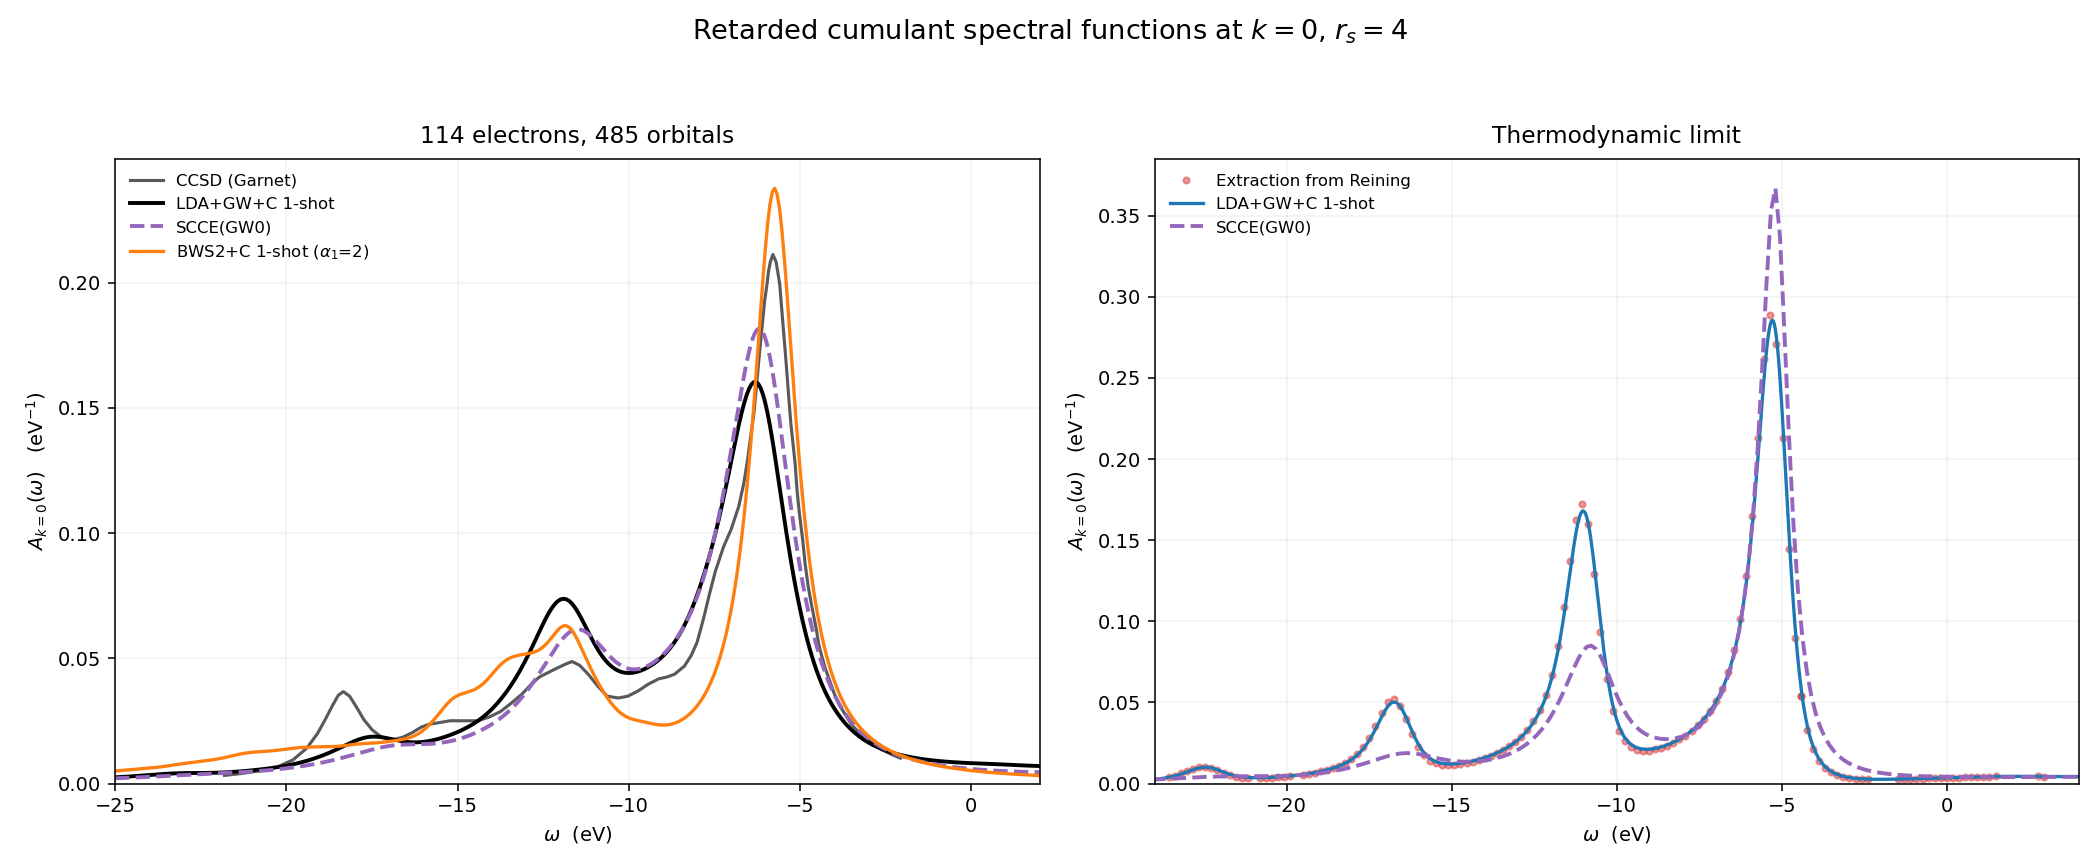
\includegraphics[width=\textwidth]{26/8/8-28/combined_k0_scce.png}
\end{figure}\pause
I should do more with this
\end{frame}
\begin{frame}
    \frametitle{scGW0}
    \begin{figure}
        \centering
        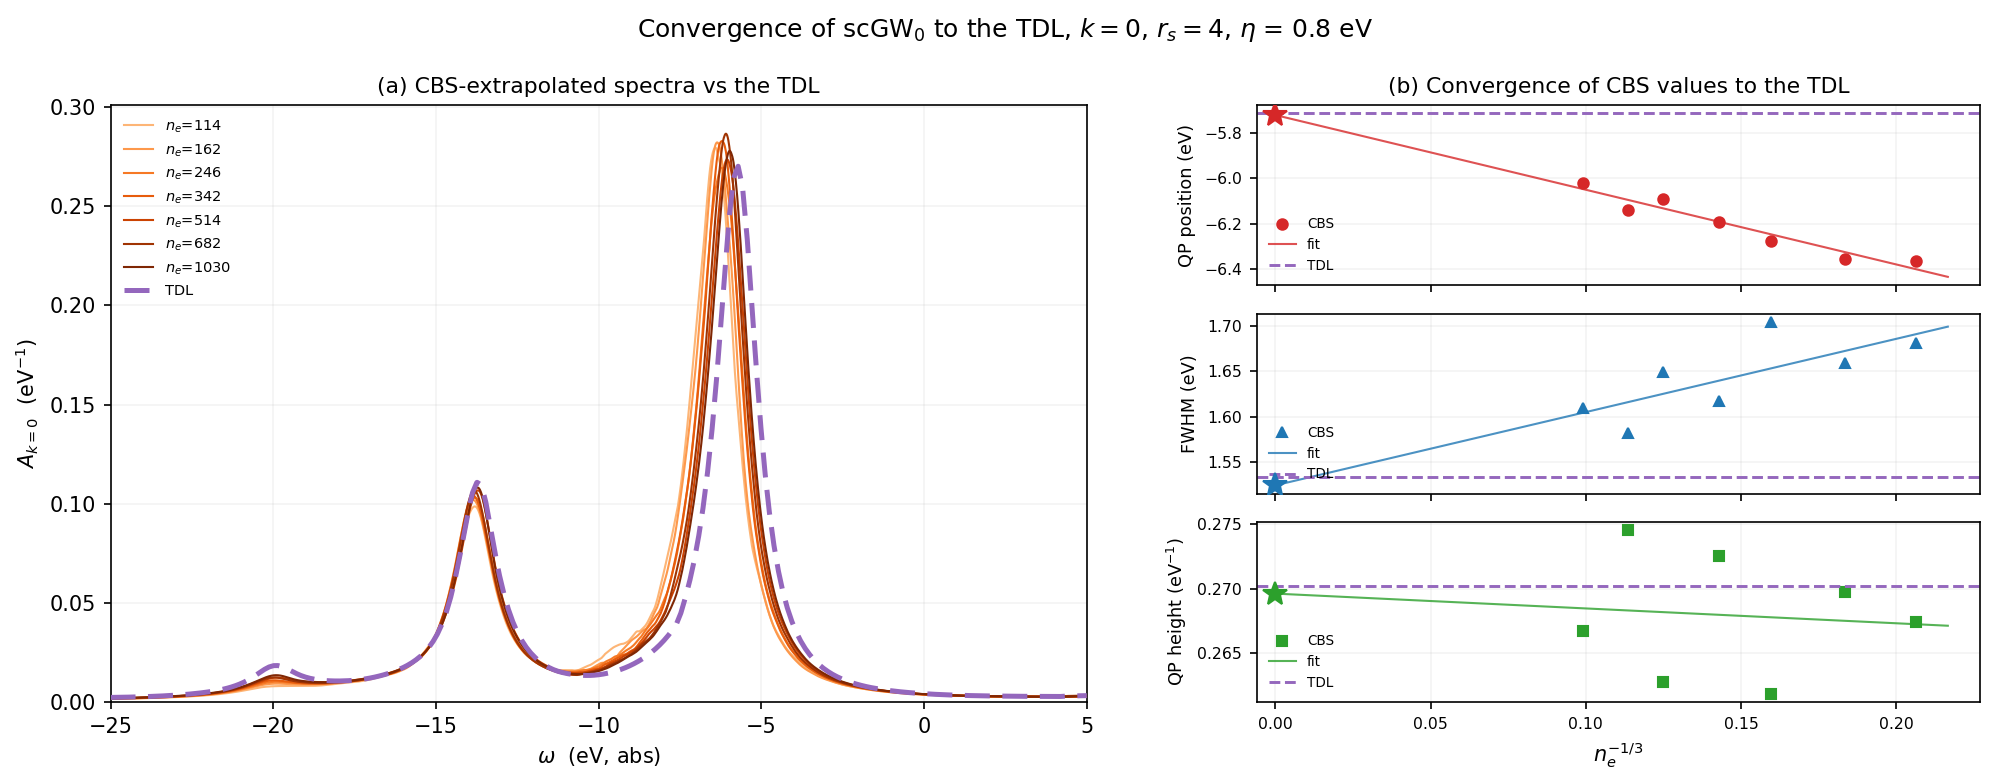
\includegraphics[width=\textwidth]{26/9/9-09/scgw0_cbs_tdl_compare_cbspm_es0.0272_tdl0.136.png}
\end{figure} \pause
    \begin{itemize}
        \item scGW has been trickier to converge \pause
         \item To show convergence rigorously, I need to do 114e up to the CBS, and only then go to TDL?
    \end{itemize}
\end{frame}
\section{Optionally review BWs2+C from my notes}

\section{Methods for the quasiboson Hamiltonian}

\begin{frame}
    \frametitle{Theory for the UEG}
\begin{align}
\hat{H}
% &=
% \hat{H}_{\rm el}
% +
% \hat{H}_{\rm pl}
% +
% \hat{H}_{\rm ep}
% \\
&=
\sum_{\bm{k}\in\mathcal{O}}
\epsilon_{\bm{k}}^{\rm HF}
a_{\bm{k}}^{\dagger}a_{\bm{k}}
+
\sum_{\nu_{\bm{q}}\in\mathcal{M}}
\omega_{\nu_{\bm{q}}}^{\rm pl}
b_{\nu_{\bm{q}}}^{\dagger}
b_{\nu_{\bm{q}}}
\nonumber\\
&\quad
+
\sum_{\bm{k},\bm{k}+\bm{q}\in\mathcal{O}}
\sum_{\nu_{\bm{q}}\in\mathcal{M}}
g_{\nu}^{\rm pl}(\bm{k},\bm{q})
a_{\bm{k}+\bm{q}}^{\dagger}
a_{\bm{k}}
\left(
b_{\nu_{-\bm{q}}}^{\dagger}
+
b_{\nu_{\bm{q}}}
\right).
\label{eq:H}
\end{align}\pause
    \begin{itemize}
        \item Three approximations to the electronic structure Hamiltonian. \pause
        \begin{itemize}
            \item Plasma oscillations within the harmonic approximation 
            \item Linear hole-plasmon coupling \pause
            \item Obtaining plasmonic quantities through linear response. \pause GW+BSE?
        \end{itemize}
    \end{itemize}
\end{frame}
\begin{frame}
    \frametitle{CC on the UEG}
\begin{itemize}
\item $(N-1)$-electron reference is
\begin{equation}
    |\Phi_0\rangle
    =
    h_{0}^{\dagger}|0\rangle_F
    \otimes
    |0\rangle_{\rm pl}
\end{equation}\pause
\item For the UEG, $\hat{T}^{(1)}=\hat{T}_{\rm ep}^{(1)}$ and $\hat{T}^{(2)}=\hat{T}_{\rm pl}^{(2)}+\hat{T}_{\rm ep}^{(2)}$\pause
\item Momentum projection is not useful \pause
\item  CC-0-S0-(1,1) is $G_0W_0$!
\end{itemize}
\end{frame}
\begin{frame}
    \frametitle{CC-0-S0-(1,1) is $G_0W_0$}
    \begin{figure}
        \centering
        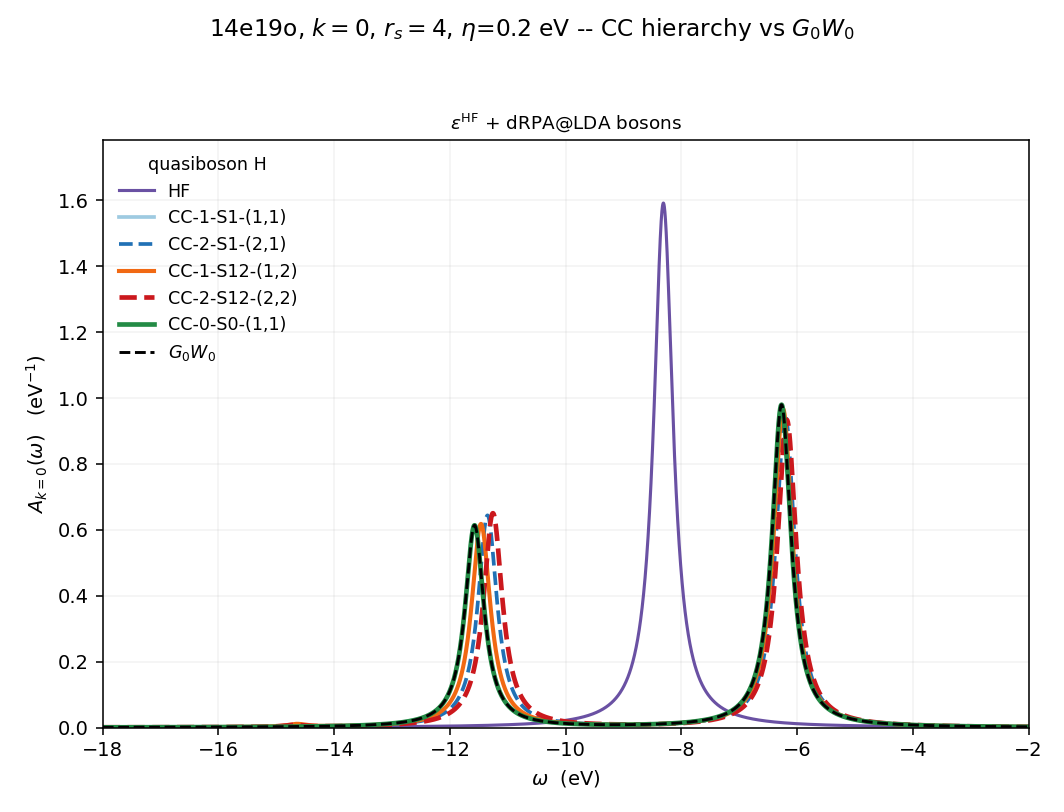
\includegraphics[width=0.9\textwidth]{26/9/9-09/k0_14e19o_drpa_lda_cc0s0_g0w0.png}
\end{figure}
\end{frame}
\begin{frame}
    \frametitle{Results for 14e19o (with PJ's SCCE)}
    \begin{figure}
        \centering
        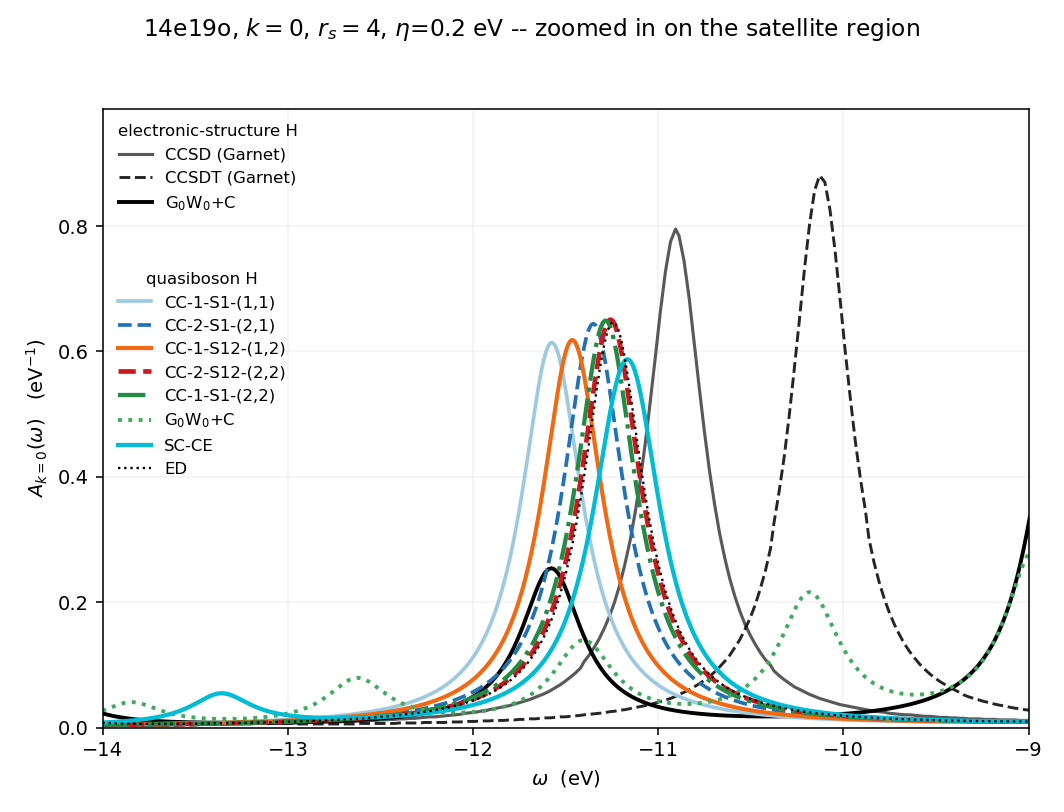
\includegraphics[width=0.9\textwidth]{26/9/9-09/k0_14e19o_drpa_lda_scce_bench_zoomm14_m9.png}
\end{figure}
\end{frame}
\begin{frame}
    \frametitle{Results for 114e485o (with PJ's SCCE)}
    \begin{figure}
        \centering
        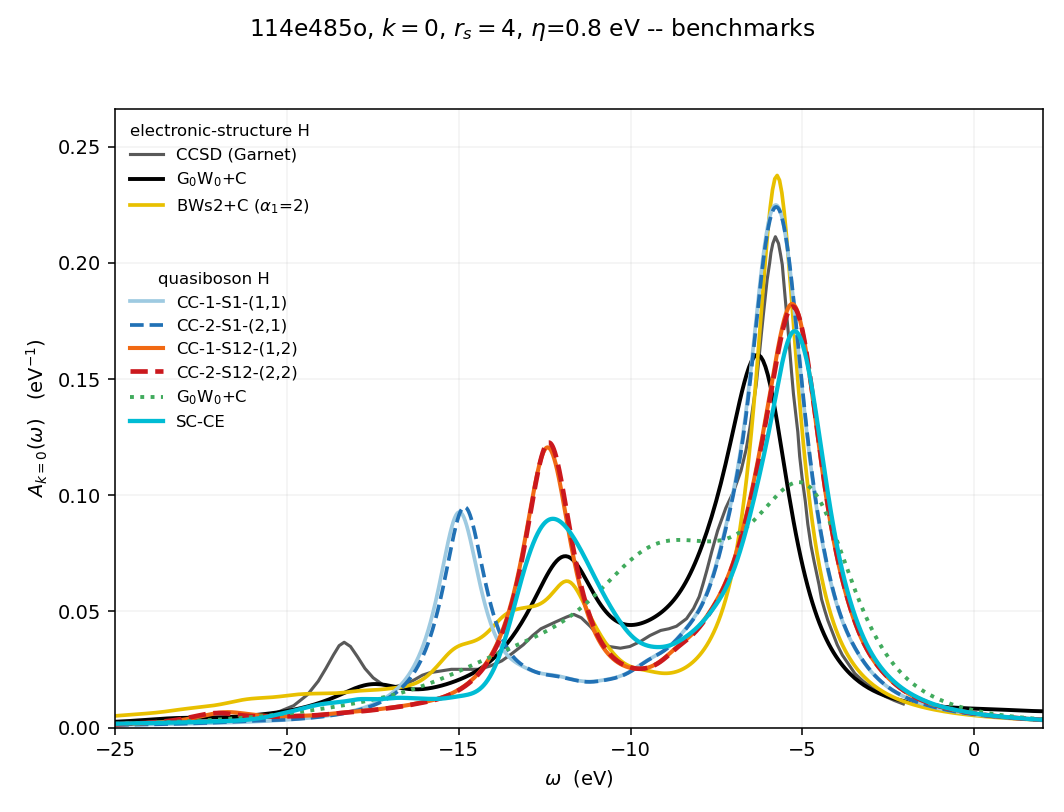
\includegraphics[width=0.9\textwidth]{26/9/9-09/k0_114e485o_drpa_lda_scce_bench.png}
\end{figure}
\end{frame}
\begin{frame}
\frametitle{Questions}
\begin{itemize}
    \item How do we expect CC and SCCE to do when we truncate the number of plasmons? \pause
    \item Does it make sense to do stochastic RI on dRPA? \pause
   \item Run all GW variants on \emph{this} quasiboson Hamiltonian? \pause
   \item Run C(2) and BWs2+C on \emph{this} quasiboson Hamiltonian to verify behavior? \pause
   \item Do we expect the quasiboson Hamiltonian to become more accurate towards the TDL? \pause
    \item Are there any other methods from the polaron literature that we should compare against?
\end{itemize}
\end{frame}
